\documentclass[12pt,a4paper,twoside]{article}
\usepackage[utf8]{inputenc}
\usepackage[finnish]{babel}
\usepackage{amsmath}
\usepackage{amsfonts}
\usepackage{amssymb}
\usepackage{graphicx}


\begin{document}

\section{Ensimmäinen}

Lorem ipsum dolor sit amet, consectetur adipiscing elit. Sed nec ligula ut mauris fermentum mollis. Praesent a gravida urna. Vivamus fermentum leo id pharetra convallis. Donec ut velit libero. Maecenas eros nisl, varius in placerat id, tincidunt ac lacus. Nam molestie varius enim cursus hendrerit. Mauris sed libero tortor. \footnote{Vestibulum at condimentum eros.}

% Tämä on kommentti.
Etiam accumsan magna magna, vel $\alpha = \sqrt[4]{x^2} = x$ mollis ligula suscipit ac. Integer vel arcu erat. Vestibulum sed nunc id orci sagittis convallis. In et ligula vitae erat volutpat dictum vel vel lorem. Quisque mauris leo, ultricies a nisl eget, tincidunt viverra risus. Aliquam congue euismod enim, finibus convallis magna cursus nec. Integer quis tempor diam. Donec hendrerit tortor et enim efficitur malesuada. Morbi venenatis sapien dolor, at lacinia arcu interdum sed.
	\begin{displaymath}
		B_{\lambda}(T) = \frac{2hc^2}{\lambda^5} \frac{1}{e^{\frac{hc}{\lambda k T}} -1 } 
	\end{displaymath}
Kun T tai $\lambda$ hyvin suuria: \\
	\begin{equation}
		B_{\lambda}(T) \approx  \frac{2hckT}{\lambda^4}
	\end{equation}
\textbf{Nunc eu nulla iaculis, fringilla justo vel, finibus magna.} Ut congue lectus vel mauris placerat, in rutrum diam dignissim. Praesent commodo, lorem eu faucibus tristique, justo magna semper ex, id gravida sapien lorem blandit odio. Quisque in vulputate turpis. Mauris finibus imperdiet velit, at auctor tortor venenatis ut. Quisque dignissim libero ex, a porta quam accumsan quis $\beta = \int  2 x \, dx = x^2 $. Fusce finibus ipsum a massa sodales, in feugiat nunc faucibus. Duis condimentum diam quis fringilla commodo. Cras vehicula rutrum volutpat. Pellentesque eleifend pulvinar interdum. Nullam at facilisis erat. \emph{Nullam euismod ultricies ullamcorper. Curabitur dignissim rhoncus nulla sed feugiat.}

\begin{enumerate}
	\item A
	\item B
	\begin{itemize}
		\item[a)] A?
		\item[b)] B?
		\item ?!
	\end{itemize}
\end{enumerate}

\newpage

\section{Toinen}

Nunc eu nulla iaculis, fringilla justo vel, finibus magna. Ut congue lectus vel mauris placerat, in rutrum diam dignissim. Praesent commodo, lorem eu faucibus tristique, justo magna semper ex, id gravida sapien lorem blandit odio. Quisque in vulputate turpis. Mauris finibus imperdiet velit, at auctor tortor venenatis ut. Quisque dignissim libero ex, a porta quam accumsan quis. Fusce finibus ipsum a massa sodales, in feugiat nunc faucibus. Duis condimentum diam quis fringilla commodo. Cras vehicula rutrum volutpat. Pellentesque eleifend pulvinar interdum. Nullam at facilisis erat. Nullam euismod ultricies ullamcorper. Curabitur dignissim rhoncus nulla sed feugiat.

\subsection{Aliotsikko}
Etiam fringilla felis ut mauris facilisis interdum. Vestibulum sagittis lectus cursus libero gravida, et tincidunt urna vehicula. Vestibulum nibh augue, blandit ac nisl ac, iaculis blandit felis. Maecenas sed faucibus arcu. Pellentesque gravida urna purus. Nulla vitae sodales ligula. Proin eleifend neque nibh, ut elementum augue vehicula placerat. In lobortis ligula eget nulla porttitor ultrices.
\begin{displaymath}
        \frac{d}{dx}\left( \int_{0}^{x} f(u)\,du\right)=f(x).
\end{displaymath}
Donec quis dui sit amet orci rhoncus malesuada. Quisque sodales maximus urna, consectetur sodales felis pretium ac. Ut elementum ex risus, id venenatis elit tincidunt sit amet. Vestibulum ante ipsum primis in faucibus orci luctus et ultrices posuere cubilia Curae; Quisque ac orci interdum, porttitor quam sit amet, ultricies eros. Suspendisse accumsan luctus justo quis pellentesque. Nulla et egestas magna. Cras facilisis sed mi nec pharetra. 

\section{Kolmas}

Lorem ipsum dolor sit amet, consectetur adipiscing elit. In eu lectus ornare, mattis elit ac, feugiat lectus. Suspendisse gravida et risus nec maximus. Integer porta dictum aliquam. Aliquam lobortis, mi at pulvinar tincidunt, nisi mi dapibus augue, eu efficitur odio sem vel leo. Vivamus et elit nunc. Aenean vehicula tristique finibus. Praesent a condimentum quam, at bibendum risus. Donec pharetra tortor ac magna viverra gravida vitae vel diam. Etiam eget hendrerit massa, eu luctus lacus. Aenean neque urna, dictum sit amet nunc nec, finibus hendrerit mi. Etiam eget dictum ex. Suspendisse quis nisi malesuada, consectetur ex ac, tempor mi. Maecenas auctor feugiat justo, in tempor augue sollicitudin in. Lorem ipsum dolor sit amet, consectetur adipiscing elit. Cras non semper ante, sit amet consectetur tortor. Duis tempus mattis mauris id commodo.

\begin{equation}
        \frac{d}{dx}\left( \int_{0}^{x} f(u)\,du\right)=f(x).
\end{equation}

Phasellus tincidunt eros vel iaculis feugiat. Curabitur ac semper arcu. Morbi vestibulum magna a venenatis vulputate. Fusce consequat gravida nibh non maximus. Pellentesque habitant morbi tristique senectus et netus et malesuada fames ac turpis egestas. Donec non sagittis tortor. Curabitur a est a lorem auctor laoreet id quis velit. Aliquam ac fermentum magna. Cras vitae laoreet ex. Aenean lectus mauris, scelerisque nec tempus gravida, pellentesque interdum ipsum. Sed dui lectus, varius a mauris sed, imperdiet molestie ligula. Nulla convallis lorem elit, sed faucibus ex mattis non. Nunc laoreet et est aliquet rhoncus. Donec vel nisi mauris. Curabitur ullamcorper vel urna eget euismod.
\begin{figure}[!t]
	\centering
		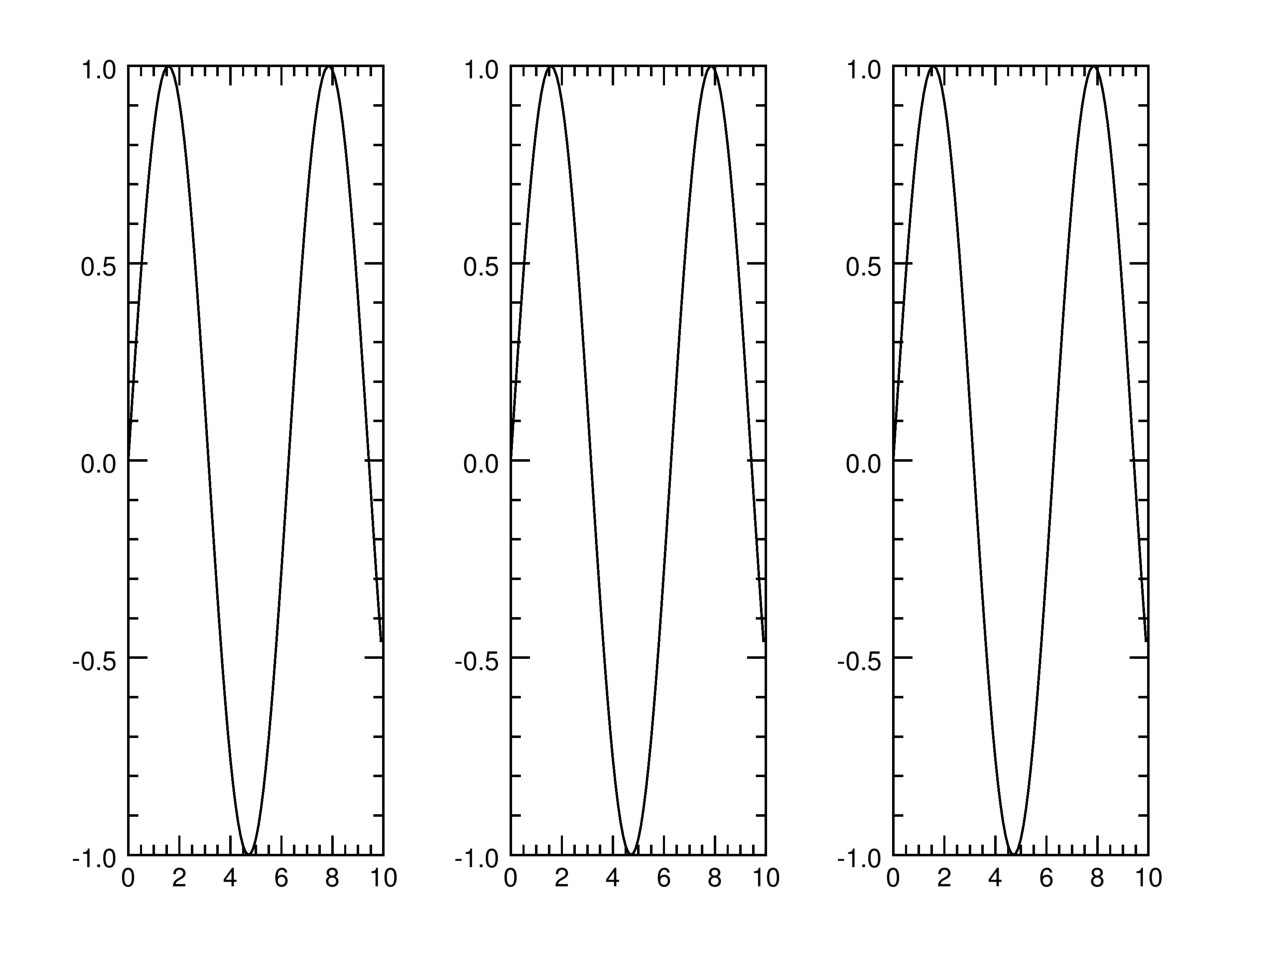
\includegraphics[width=\textwidth]{sini.pdf}
		\caption{Sini.}
\end{figure}
Duis porta, metus sed bibendum volutpat, diam ipsum blandit sem, eu scelerisque mi neque sit amet lectus. Fusce malesuada faucibus quam quis suscipit. Etiam fringilla ante ipsum, vel fermentum libero ultrices id. Nam laoreet quam quis velit pulvinar eleifend. Donec ornare mauris ac lorem condimentum, a volutpat sem iaculis. Quisque feugiat velit risus, a rutrum risus sollicitudin eget. Nunc eget magna posuere, molestie dolor quis, tristique erat. In rhoncus vestibulum sagittis. 

\begin{center}
	\begin{tabular}{l | l c c c}
			&	Tähden nimi & Etäisyys [pc] & Spektriluokka & Absoluuttinen kirkkaus \\
			\hline
		1. & Aurinko & 	0 & G2V & 4.85 \\
		2. & Proxima Centauri & 1.3 & M5.5Ve & 15.53 \\
		3. & $\alpha$ Centauri A & 1.34 & G2V & 4.38 \\
		4. & $\alpha$ Centauri B & 1.34 & K1V & 5.71 \\
		5. & Barnardin tähti & 1.83 & M4.0Ve & 13.22 \\
		6. & Luhman 16A & 2.02 & L8 & NA \\
		7. & Luhman 16B & 2.02 & T1 & NA \\
		8. & Wise 0855-0714 & 2.21 & Y & NA \\
		9. & Lalande 21185 & 2.54 & M6.0V & 16.55 \\
		10. & Sirius A & 2.63 & A1V & 1.42 						
	\end{tabular}					
\end{center}

\end{document}